\chapter{Datos de Panel}

El dato verdadero de panel se trata de tener una serie continua a lo largo del tiempo, esto a diferencia de los datos pooled cross-section, que se trata de poner un dato debajo de otro.

$$y_{it} = \beta_0+\beta_1x_{it1}+\cdots + \beta_k x_{itk} + u_{it}$$

Donde:

\begin{itemize}
	\item $t= 1,2,\cdots, T$ es el tiempo.
	\item $i= 1,2,\cdots, N$ es el número de unidades.
\end{itemize}

Existen dos clases de paneles:

\begin{itemize}
    \item Paneles micro. Siempre que $t<N$. (30000 empresas y 10 años).
    \item Paneles macro. Siempre que $t\approx N$. (30 países y 30 años).
\end{itemize}

Un panel es \textbf{balanceado} si todas las unidades tienen la misma cantidad de observaciones. Y es \textbf{desbalanceado} si no todas las unidades tienen la misma cantidad de observaciones.

Con respecto a pooled cross-section,
\begin{itemize}
    \item Lo utilizamos para investigar el efecto del tiempo.
    \item Lo utilizaremos si hay relaciones en el tiempo.
\end{itemize}

\section{Chapter 13: Pooling Cross-Sections Across Time, Simple Panel Data Methods}

En este ejemplo responderemos a:
\begin{center}
    ¿Ha variado la fertilidad de las mujeres en el tiempo?
\end{center}

Utilizaremos datos de 1129 mujeres, que le preguntaremos cuantos hijos tiene. Tendremos datos para 7 años cada 2 años. Colocaremos las variables ficticias para no entrar en la trampa de variables ficticias.

\subsection{Variables ficticias}
Nunca podemos poner todas las categorías al mismo tiempo, ya que tendríamos multicolinialidad exacta. Por lo que al aplicar MCO no podríamos estimar los coeficientes.

\begin{center}
Modelo 1: MCO, usando las observaciones 1--1129\\
Variable dependiente: kids\\

\vspace{1em}

\begin{tabular}{lr@{,}lr@{,}lr@{,}lr@{,}l}
  &
 \multicolumn{2}{c}{Coeficiente} &
  \multicolumn{2}{c}{Desv.\ Típica} &
   \multicolumn{2}{c}{Estadístico $t$} &
    \multicolumn{2}{c}{valor p} \\[1ex]
const &
  $-$7&74246 &
    3&05177 &
      $-$2&537 &
        0&0113 \\
educ &
  $-$0&128427 &
    0&0183486 &
      $-$6&999 &
        0&0000 \\
age &
  0&532135 &
    0&138386 &
      3&845 &
        0&0001 \\
agesq &
  $-$0&00580400 &
    0&00156428 &
      $-$3&710 &
        0&0002 \\
black &
  1&07566 &
    0&173536 &
      6&198 &
        0&0000 \\
east &
  0&217324 &
    0&132788 &
      1&637 &
        0&1020 \\
northcen &
  0&363114 &
    0&120897 &
      3&004 &
        0&0027 \\
west &
  0&197603 &
    0&166913 &
      1&184 &
        0&2367 \\
farm &
  $-$0&0525575 &
    0&147190 &
      $-$0&3571 &
        0&7211 \\
othrural &
  $-$0&162854 &
    0&175442 &
      $-$0&9282 &
        0&3535 \\
town &
  0&0843532 &
    0&124531 &
      0&6774 &
        0&4983 \\
smcity &
  0&211879 &
    0&160296 &
      1&322 &
        0&1865 \\
y74 &
  0&268183 &
    0&172716 &
      1&553 &
        0&1208 \\
y76 &
  $-$0&0973795 &
    0&179046 &
      $-$0&5439 &
        0&5866 \\
y78 &
  $-$0&0686665 &
    0&181684 &
      $-$0&3779 &
        0&7055 \\
y80 &
  $-$0&0713053 &
    0&182771 &
      $-$0&3901 &
        0&6965 \\
y82 &
  $-$0&522484 &
    0&172436 &
      $-$3&030 &
        0&0025 \\
y84 &
  $-$0&545166 &
    0&174516 &
      $-$3&124 &
        0&0018 \\
\end{tabular}

\vspace{1ex}
\begin{tabular}{lrlr}
Media de la vble. dep. &  2,743136 & D.T. de la vble. dep. &  1,653899 \\
Suma de cuad. residuos &  2685,898 & D.T. de la regresión &  1,554847 \\
$R^2$ &  0,129512 & $R^2$ corregido &  0,116192 \\
$F(17, 1111)$ &  9,723282 & Valor p (de $F$) &  2,42\textrm{e--24} \\
Log-verosimilitud & $-$2091,224 & Criterio de Akaike &  4218,448 \\
Criterio de Schwarz &  4308,972 & Hannan--Quinn &  4252,650 \\
\end{tabular}
\end{center}

% importar imagen
\begin{center}
    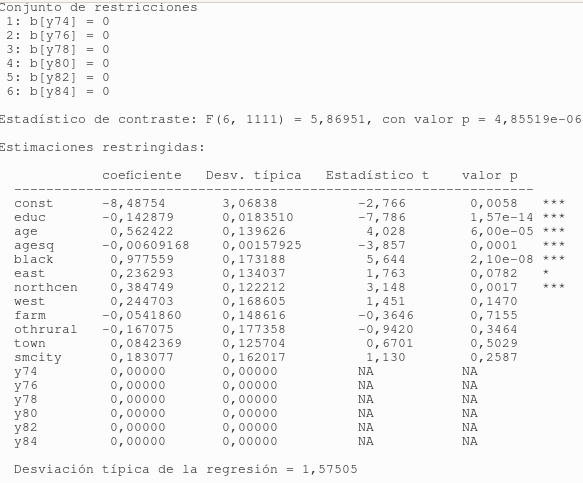
\includegraphics[scale = .5]{./image/kids_contraste_gretl.png}
\end{center}

Se rechaza la hipótesis nula de que los coeficientes de las variables ficticias son iguales a 0. Por lo que se rechaza la hipótesis nula de que la fertilidad de las mujeres no ha variado en el tiempo.


\section{Ejemplo 13.2}

\begin{center}
    ¿Podemos encontrar diferencias salariales por género según la educación?
\end{center}

Serán datos para 78 y 85. Trataremos de predecir los salarios.

\subsection{Efectos de interacción}


\begin{center}

Modelo 1: MCO, usando las observaciones 1--1084\\
Variable dependiente: lwage\\

\vspace{1em}

\begin{tabular}{lr@{,}lr@{,}lr@{,}lr@{,}l}
  &
 \multicolumn{2}{c}{Coeficiente} &
  \multicolumn{2}{c}{Desv.\ Típica} &
   \multicolumn{2}{c}{Estadístico $t$} &
    \multicolumn{2}{c}{valor p} \\[1ex]
const &
  0&458933 &
    0&0934485 &
      4&911 &
        0&0000 \\
y85 &
  0&117806 &
    0&123782 &
      0&9517 &
        0&3415 \\
educ &
  0&0747209 &
    0&00667643 &
      11&19 &
        0&0000 \\
y85edu &
  0&0184605 &
    0&00935417 &
      1&974 &
        0&0487 \\
exper &
  0&0295843 &
    0&00356731 &
      8&293 &
        0&0000 \\
expersq &
  $-$0&000399428 &
    7&75391\textrm{e--05} &
      $-$5&151 &
        0&0000 \\
union &
  0&202132 &
    0&0302945 &
      6&672 &
        0&0000 \\
female &
  $-$0&316709 &
    0&0366214 &
      $-$8&648 &
        0&0000 \\
y85fem &
  0&0850520 &
    0&0513090 &
      1&658 &
        0&0977 \\
\end{tabular}

\vspace{1ex}
\begin{tabular}{lrlr}
Media de la vble. dep. &  1,867301 & D.T. de la vble. dep. &  0,542804 \\
Suma de cuad. residuos &  183,0991 & D.T. de la regresión &  0,412704 \\
$R^2$ &  0,426186 & $R^2$ corregido &  0,421915 \\
$F(8, 1075)$ &  99,80353 & Valor p (de $F$) &  4,5\textrm{e--124} \\
Log-verosimilitud & $-$574,2443 & Criterio de Akaike &  1166,489 \\
Criterio de Schwarz &  1211,384 & Hannan--Quinn &  1183,485 \\
\end{tabular}
\end{center}

Dado que female es negativo, existe un efecto negativo en los salarios. 

En el año base 78, ser mujer disminuye el salario en 0.3. En el año 85, ser mujer es -0.3+0.08 = -0.22. Por lo que el efecto de ser mujer aumenta en 0.08.

La educación tiene un efecto positivo en el salario en el año 78. Ahora ¿Es más importante estudiar en el año 85 o en el 78?: Es mas importante estudiar en el año 85, ya que el efecto de la educación se refuerza en 0.018.

\section{Diferencias en diferencias}

\begin{itemize}
    \item Un experimento natural es por ejemplo los experimentos médicos, donde el existe un grupo de control y un grupo de tratamiento.
    \item En economía, un experimento natural es por ejemplo el efecto de un cambio en la política económica, donde se compara un grupo de control y un grupo de tratamiento.
    \item Debemos añadir variables adicionales, para controlar las diferencias entre el grupo de control y el grupo de tratamiento.
\end{itemize}

\section{Ejemplo 13.3}

\begin{center}
	¿Cuál es el efecto de un incinerador de basura en el precio de las casas?
\end{center}

Recordemos que necesitamos dos variables ficticias, una para el grupo de tratamiento y otra para el grupo de control.
$$y_{it} = \beta_0 + \beta_1 treatment_{it} + \beta_2 after_{it} + \beta_3 treatment_{it} after_{it} + u_{it}$$
Es decir, una que sera treatment y otra que sera after.

El after mide el periodo = 1 tiempo 1 y el periodo = 0 tiempo 2. Será antes de construir el incinerador y después de construir el incinerador.\\

También necesitamos los que hay recibido el tratamiento y los que no han recibido el tratamiento. Cómo, treatment = 1 y treatment = 0. En nuestro caso, casas cerca del incinerador y casas lejos del incinerador.\\

Para ello veremos si hay evidencia estadísticamente significativa de cambios en los precios por el hecho de antes y después de la construcción del incinerador. Cómo también se verá la diferencia entre antes y después de la construcción del incinerador en las casas cerca del incinerador y las casas lejos del incinerador.
$$\left(y_{2,B}-y_{2,A}\right)-\left(y_{1,B}+y_{1,A}\right) \quad \text{o} \quad \left(y_{2,B}-y_{1,VBB}\right)-\left(y_{2,A}-y_{1,A}\right)$$

Con mínimos cuadrados ordinarios tenemos

\begin{center}

Modelo 1: MCO, usando las observaciones 1--321\\
Variable dependiente: rprice\\

\vspace{1em}

\begin{tabular}{lr@{,}lr@{,}lr@{,}lr@{,}l}
  &
 \multicolumn{2}{c}{Coeficiente} &
  \multicolumn{2}{c}{Desv.\ Típica} &
   \multicolumn{2}{c}{Estadístico $t$} &
    \multicolumn{2}{c}{valor p} \\[1ex]
const &
  82517&2 &
    2726&91 &
      30&26 &
        0&0000 \\
y81 &
  18790&3 &
    4050&07 &
      4&640 &
        0&0000 \\
nearinc &
  $-$18824&4 &
    4875&32 &
      $-$3&861 &
        0&0001 \\
y81nrinc &
  $-$11863&9 &
    7456&65 &
      $-$1&591 &
        0&1126 \\
\end{tabular}

\vspace{1ex}
\begin{tabular}{lrlr}
Media de la vble. dep. &  83721,36 & D.T. de la vble. dep. &  33118,79 \\
Suma de cuad. residuos &  2,90\textrm{e+11} & D.T. de la regresión &  30242,90 \\
$R^2$ &  0,173948 & $R^2$ corregido &  0,166131 \\
$F(3, 317)$ &  22,25107 & Valor p (de $F$) &  4,22\textrm{e--13} \\
Log-verosimilitud & $-$3765,229 & Criterio de Akaike &  7538,458 \\
Criterio de Schwarz &  7553,544 & Hannan--Quinn &  7544,481 \\
\end{tabular}


\end{center}

Todas las variables son estadísticamente significativas. 

\begin{itemize}
    \item Para $y81nrinc$, Aquellas casas que están cerca del incinerador y después que se construyeron, hay una reducción del precio.
\end{itemize}

Dado que para las políticas publicas no se realizó aleatoriamente la distribución de casas, podemos añadir otras variables explicativas como la edad y la edad al cuadrado de las casas.


\begin{center}

Modelo 2: MCO, usando las observaciones 1--321\\
Variable dependiente: rprice\\

\vspace{1em}

\begin{tabular}{lr@{,}lr@{,}lr@{,}lr@{,}l}
  &
 \multicolumn{2}{c}{Coeficiente} &
  \multicolumn{2}{c}{Desv.\ Típica} &
   \multicolumn{2}{c}{Estadístico $t$} &
    \multicolumn{2}{c}{valor p} \\[1ex]
const &
  89116&5 &
    2406&05 &
      37&04 &
        0&0000 \\
y81 &
  21321&0 &
    3443&63 &
      6&191 &
        0&0000 \\
nearinc &
  9397&94 &
    4812&22 &
      1&953 &
        0&0517 \\
y81nrinc &
  $-$21920&3 &
    6359&75 &
      $-$3&447 &
        0&0006 \\
age &
  $-$1494&42 &
    131&860 &
      $-$11&33 &
        0&0000 \\
agesq &
  8&69128 &
    0&848127 &
      10&25 &
        0&0000 \\
\end{tabular}

\vspace{1ex}
\begin{tabular}{lrlr}
Media de la vble. dep. &  83721,36 & D.T. de la vble. dep. &  33118,79 \\
Suma de cuad. residuos &  2,06\textrm{e+11} & D.T. de la regresión &  25543,29 \\
$R^2$ &  0,414448 & $R^2$ corregido &  0,405154 \\
$F(5, 315)$ &  44,59083 & Valor p (de $F$) &  1,00\textrm{e--34} \\
Log-verosimilitud & $-$3710,001 & Criterio de Akaike &  7432,001 \\
Criterio de Schwarz &  7454,630 & Hannan--Quinn &  7441,036 \\
\end{tabular}


\end{center}


\begin{itemize}
    \item Para $y8lnrinc$, vemos que ya es estadísticamente significativo, por lo que la construcción del incinerador tiene un efecto negativo en el precio de las casas después de que se construyó el incinerador ($81$).
\end{itemize}


Hay otras maneras de introducir variables ficticias como:


\begin{center}

Modelo 3: MCO, usando las observaciones 1--321\\
Variable dependiente: rprice\\

\vspace{1em}

\begin{tabular}{lr@{,}lr@{,}lr@{,}lr@{,}l}
  &
 \multicolumn{2}{c}{Coeficiente} &
  \multicolumn{2}{c}{Desv.\ Típica} &
   \multicolumn{2}{c}{Estadístico $t$} &
    \multicolumn{2}{c}{valor p} \\[1ex]
const &
  5204&92 &
    12145&7 &
      0&4285 &
        0&6686 \\
y81 &
  18881&3 &
    2980&04 &
      6&336 &
        0&0000 \\
nearinc &
  7636&99 &
    4837&66 &
      1&579 &
        0&1154 \\
y81nrinc &
  $-$15969&7 &
    5445&18 &
      $-$2&933 &
        0&0036 \\
age &
  $-$670&725 &
    142&997 &
      $-$4&690 &
        0&0000 \\
agesq &
  3&48603 &
    0&888372 &
      3&924 &
        0&0001 \\
intst &
  $-$0&476274 &
    0&214412 &
      $-$2&221 &
        0&0271 \\
land &
  0&154049 &
    0&0339211 &
      4&541 &
        0&0000 \\
rooms &
  5852&16 &
    1780&63 &
      3&287 &
        0&0011 \\
baths &
  17233&5 &
    2432&46 &
      7&085 &
        0&0000 \\
\end{tabular}

\vspace{1ex}
\begin{tabular}{lrlr}
Media de la vble. dep. &  83721,36 & D.T. de la vble. dep. &  33118,79 \\
Suma de cuad. residuos &  1,43\textrm{e+11} & D.T. de la regresión &  21442,87 \\
$R^2$ &  0,592594 & $R^2$ corregido &  0,580804 \\
$F(9, 311)$ &  50,26293 & Valor p (de $F$) &  1,58\textrm{e--55} \\
Log-verosimilitud & $-$3651,780 & Criterio de Akaike &  7323,560 \\
Criterio de Schwarz &  7361,275 & Hannan--Quinn &  7338,619 \\
\end{tabular}


\end{center}

OTRO Ejemplo


\begin{center}

Modelo 4: MCO, usando las observaciones 1--321\\
Variable dependiente: lrprice\\

\vspace{1em}

\begin{tabular}{lr@{,}lr@{,}lr@{,}lr@{,}l}
  &
 \multicolumn{2}{c}{Coeficiente} &
  \multicolumn{2}{c}{Desv.\ Típica} &
   \multicolumn{2}{c}{Estadístico $t$} &
    \multicolumn{2}{c}{valor p} \\[1ex]
const &
  8&80179 &
    0&294228 &
      29&91 &
        0&0000 \\
y81 &
  0&239526 &
    0&0413352 &
      5&795 &
        0&0000 \\
nearinc &
  $-$0&0489247 &
    0&0600863 &
      $-$0&8142 &
        0&4161 \\
y81nrinc &
  $-$0&161399 &
    0&0763260 &
      $-$2&115 &
        0&0352 \\
lland &
  0&231838 &
    0&0273442 &
      8&479 &
        0&0000 \\
\end{tabular}

\vspace{1ex}
\begin{tabular}{lrlr}
Media de la vble. dep. &  11,26138 & D.T. de la vble. dep. &  0,387900 \\
Suma de cuad. residuos &  29,57740 & D.T. de la regresión &  0,305940 \\
$R^2$ &  0,385713 & $R^2$ corregido &  0,377937 \\
$F(4, 316)$ &  49,60437 & Valor p (de $F$) &  2,26\textrm{e--32} \\
Log-verosimilitud & $-$72,77815 & Criterio de Akaike &  155,5563 \\
Criterio de Schwarz &  174,4135 & Hannan--Quinn &  163,0855 \\
\end{tabular}


\end{center}


Con esto podemos evaluar el efecto de POLÍTICAS PÚBLICAS. Una politicá pública es: ¿Donde vamos a construir el incinerador.?

\section{Dos periodos de datos de panel}

¿Cómo saber si nos olvidamos de una variables relevante? o ¿que introducimos una irrelevante?. Significa que todos mis estimadores son sesgados, o el sesgo por haber omitido variables relevantes. Es de los principales problemas que tiene la econometría. Sólo en datos de panel nos permite omitir estas variables relevantes. Supongamos que tenemos un modelo:
$$y_{it} = \beta_0 + \delta_0 d2_t + \beta_1 x_{u1} + \cdots + \beta_k x_{itk} + a_i + u_{it}.$$

Donde: $d2_t=0$ cuando $t=1$ y $d2_t=1$ cuando $t=2$. La $a_i$ pueden ser muchas variables que me puedo olvidar, constante en el tiempo.\\

Si la $a_i$ esta correlacionado con las $x$ será sesgado con mínimos cuadrados ordinarios. Intentaremos eliminar ese problema diferenciando. Es decir,

$$ t = 1 \rightarrow y_{i1} = \beta_0 + \beta_1 x_{i1} +\cdots + + \beta_k x_{ilk} + a_i + u_{i1}$$
$$ t = 2 \rightarrow y_{i2} = \beta_0 + \delta_0 + \beta_1 x_{i1} + \cdots + \beta_k x_{ik} + a_i + u_{i2}$$

Ahora tomamos la diferencia de un periodo a otro, llamada la ecuación de primeras diferencias:

$$\Delta y_i  = y_{i2} - y_{i1} = \delta_0 + \Delta \beta_i x_{i1}  + \cdots + \beta_k \Delta x_{ik} + \Delta a_i + \Delta u_i$$

POR LO TANTO $a_i$ DESAPARECE. Por lo tanto ya no tiene correlación entre las $x$ y el error.\\

Ahora aplicamos MCO a la ecuación de primeras diferencias, se le llama estimador de primeras diferencias.\\


\subsection{Ejemplo 13.5}

\textbf{¿Mientras más trabajas menos duermes?}\\

\begin{itemize}
    \item $cslonap$ número de minutos de sueño por semana. $C$ al priniipio significa primeras diferencias. Es decir, cuanto dormía en el año 85 menos cuanto dormía en el año 75.
    \item $ctotwrk$ número de horas trabajadas. $c$ diferenciado.
    \item Tenemos datos de años dormidos de dos años, 1975 y 1981.
\end{itemize}

Se debe aplicar a todas las variables la primera diferencia.\\

\begin{center}

Modelo 1: MCO, usando las observaciones 1--239\\
Variable dependiente: cslpnap\\

\vspace{1em}

\begin{tabular}{lr@{,}lr@{,}lr@{,}lr@{,}l}
  &
 \multicolumn{2}{c}{Coeficiente} &
  \multicolumn{2}{c}{Desv.\ Típica} &
   \multicolumn{2}{c}{Estadístico $t$} &
    \multicolumn{2}{c}{valor p} \\[1ex]
const &
  $-$92&6340 &
    45&8659 &
      $-$2&020 &
        0&0446 \\
ctotwrk &
  $-$0&226669 &
    0&0360540 &
      $-$6&287 &
        0&0000 \\
ceduc &
  $-$0&0244717 &
    48&7594 &
      $-$0&0005019 &
        0&9996 \\
cmarr &
  104&214 &
    92&8554 &
      1&122 &
        0&2629 \\
cyngkid &
  94&6654 &
    87&6525 &
      1&080 &
        0&2813 \\
cgdhlth &
  87&5778 &
    76&5991 &
      1&143 &
        0&2541 \\
\end{tabular}

\vspace{1ex}
\begin{tabular}{lrlr}
Media de la vble. dep. & $-$52,65690 & D.T. de la vble. dep. &  642,2038 \\
Suma de cuad. residuos &  83482612 & D.T. de la regresión &  598,5770 \\
$R^2$ &  0,149502 & $R^2$ corregido &  0,131251 \\
$F(5, 233)$ &  8,191418 & Valor p (de $F$) &  3,83\textrm{e--07} \\
Log-verosimilitud & $-$1864,387 & Criterio de Akaike &  3740,773 \\
Criterio de Schwarz &  3761,632 & Hannan--Quinn &  3749,179 \\
\end{tabular}


\end{center}

\begin{itemize}
    \item $ctotwrk$: A mayor minutos dormidos a la semana menos horas trabajadas. Estadísticamente significativo.
    \item \textbf{Puedo haberme olvidado de características de las personas, que son iguales en los dos años}.
\end{itemize}


\subsection{Ejemplo 13.7}
\textbf{¿Hay manera de poder ver el efecto de las leyes sobre la gente que conduce borracha?, ¿son efectivas para evitar los accidentes?}\\

\begin{itemize}
    \item cdthrte: tasa de muertes por accidentes de tráfico.
    \item copen: Es ilegal tener bebidas alcohólicas en el coche abiertas.
    \item cadmn: Si te para la policía, y estas borracho, se te quita la licencia. 0 si el estado tiene la ley y 1 si no tiene la ley.
    \item Años 1985 y 1990.
\end{itemize}



\begin{center}

Modelo 1: MCO, usando las observaciones 1--51\\
Variable dependiente: cdthrte\\

\vspace{1em}

\begin{tabular}{lr@{,}lr@{,}lr@{,}lr@{,}l}
  &
 \multicolumn{2}{c}{Coeficiente} &
  \multicolumn{2}{c}{Desv.\ Típica} &
   \multicolumn{2}{c}{Estadístico $t$} &
    \multicolumn{2}{c}{valor p} \\[1ex]
const &
  $-$0&496787 &
    0&0524256 &
      $-$9&476 &
        0&0000 \\
copen &
  $-$0&419679 &
    0&205595 &
      $-$2&041 &
        0&0467 \\
cadmn &
  $-$0&150602 &
    0&116822 &
      $-$1&289 &
        0&2035 \\
\end{tabular}

\vspace{1ex}
\begin{tabular}{lrlr}
Media de la vble. dep. & $-$0,545098 & D.T. de la vble. dep. &  0,358505 \\
Suma de cuad. residuos &  5,663695 & D.T. de la regresión &  0,343502 \\
$R^2$ &  0,118666 & $R^2$ corregido &  0,081944 \\
$F(2, 48)$ &  3,231444 & Valor p (de $F$) &  0,048236 \\
Log-verosimilitud & $-$16,32326 & Criterio de Akaike &  38,64652 \\
Criterio de Schwarz &  44,44200 & Hannan--Quinn &  40,86115 \\
\end{tabular}


\end{center}

\begin{itemize}
    \item $copen$: Es más efectiva que $cadmn$. Ya que $copen$ es estadísticamente significativo y $cadmn$ no lo es. Y $copen$ es más efectiva para reducir la tasa de muertes por accidentes de tráfico.
\end{itemize}


\section{Multiples periodos de datos de panel}

\begin{itemize}
    \item Si tenemos 3 periodos debemos diferenciar 1 del 2, el 2 del 3. Donde, siempre se tendrá una menos.
\end{itemize}

\subsection{Ejemplo 13.8}

\textbf{¿Puedo reducir el solicitud de desempleo?}

\begin{itemize}
    \item $guclms$: Número de solicitudes por prestación de desempleo.
    \item 22 ciudades.
    \item Tenemos datos del 80 al año 88.
    \item Al aplicar las primeras diferencias eliminamos una observación.
    \item $cez$: Zona empresarial. Ventajas fiscales para las empresas. 
\end{itemize}


\begin{itemize}
    \item 
\end{itemize}

